\question{Газовые лазеры. Лазеры на N2}
Азотный лазер работает в УФ-диапазоне. Наибольшее значение имеет длина волны 
337,1 нм. Инверсия создаётся в импульсном электрическом разряде на переходах 
между относительно высоко расположенными возбуждёнными электронными термами 
молекулы \( N_2 \). Электроны разряда в соответствии с принципом 
Франка-Кондона при вертикальных переходах столкновительно заселяют верхний, 
но относительно неразрыхлённый терм, содержащий верхние лазерные уровни. При 
этом более рыхлый терм, содержащий нижние лазерные уровни и расположенный 
правее, не заселяется. Излучение, также в соответствии с принципом 
Франка-Кондона, осуществлется при радиационных вертикальных переходах из 
правых поворотных точек верхнего терма на нижний.

\begin{figure}[h]
    \center
    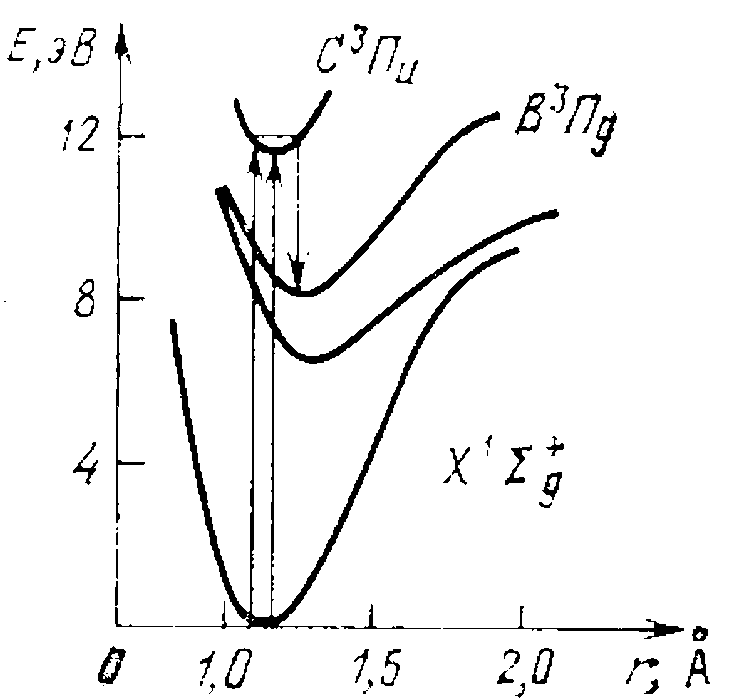
\includegraphics[width=.47\textwidth]{24}
    \caption{Уровни энергии азота}
\end{figure}

Нижние уровни обладают большим временем жизни, чем верхние, поэтому этот лазер 
относят к лазерам на самоограниченных переходах. Время существования инверсии 
в них мало (3-10 нс), поэтому она создаётся бегущей волной возбуждения, 
синхронно с импульсом света вдоль оси лазера. В силу малого времени 
существования инверсии этот лазер относят к суперлюминесцентным.

Характерным для этого лазера является разнесение каналов возбуждения и 
излучения в соответствии с принципом Франка-Кондона для переходов между 
электронными термами молекул.